%
\documentclass[10pt,a4paper]{article}


\usepackage{array}
\usepackage{subfigure}
\usepackage{graphicx}
\usepackage{amssymb}
\usepackage{amsmath}
\usepackage{cite}
\usepackage{color}
\usepackage{url}
\usepackage[lined,linesnumbered,ruled,norelsize]{algorithm2e}
\usepackage{listings}
\lstset{
  language=Octave, 
  basicstyle=\footnotesize, 
  frame=single, 
  showspaces=false, 
  showstringspaces=false}
\date{}




\begin{document}

\title{Technical Report 3: Logistic Regression and Newton's Method}

\maketitle

\section{Plot The Data}
%
  The data set and the decision boundary are illustrated in Fig.~\ref{fig:data}. It can be observed that, the boundary well separates the positive data samples from the negative ones.
  %
  \begin{figure}[htb!]
  \centering
    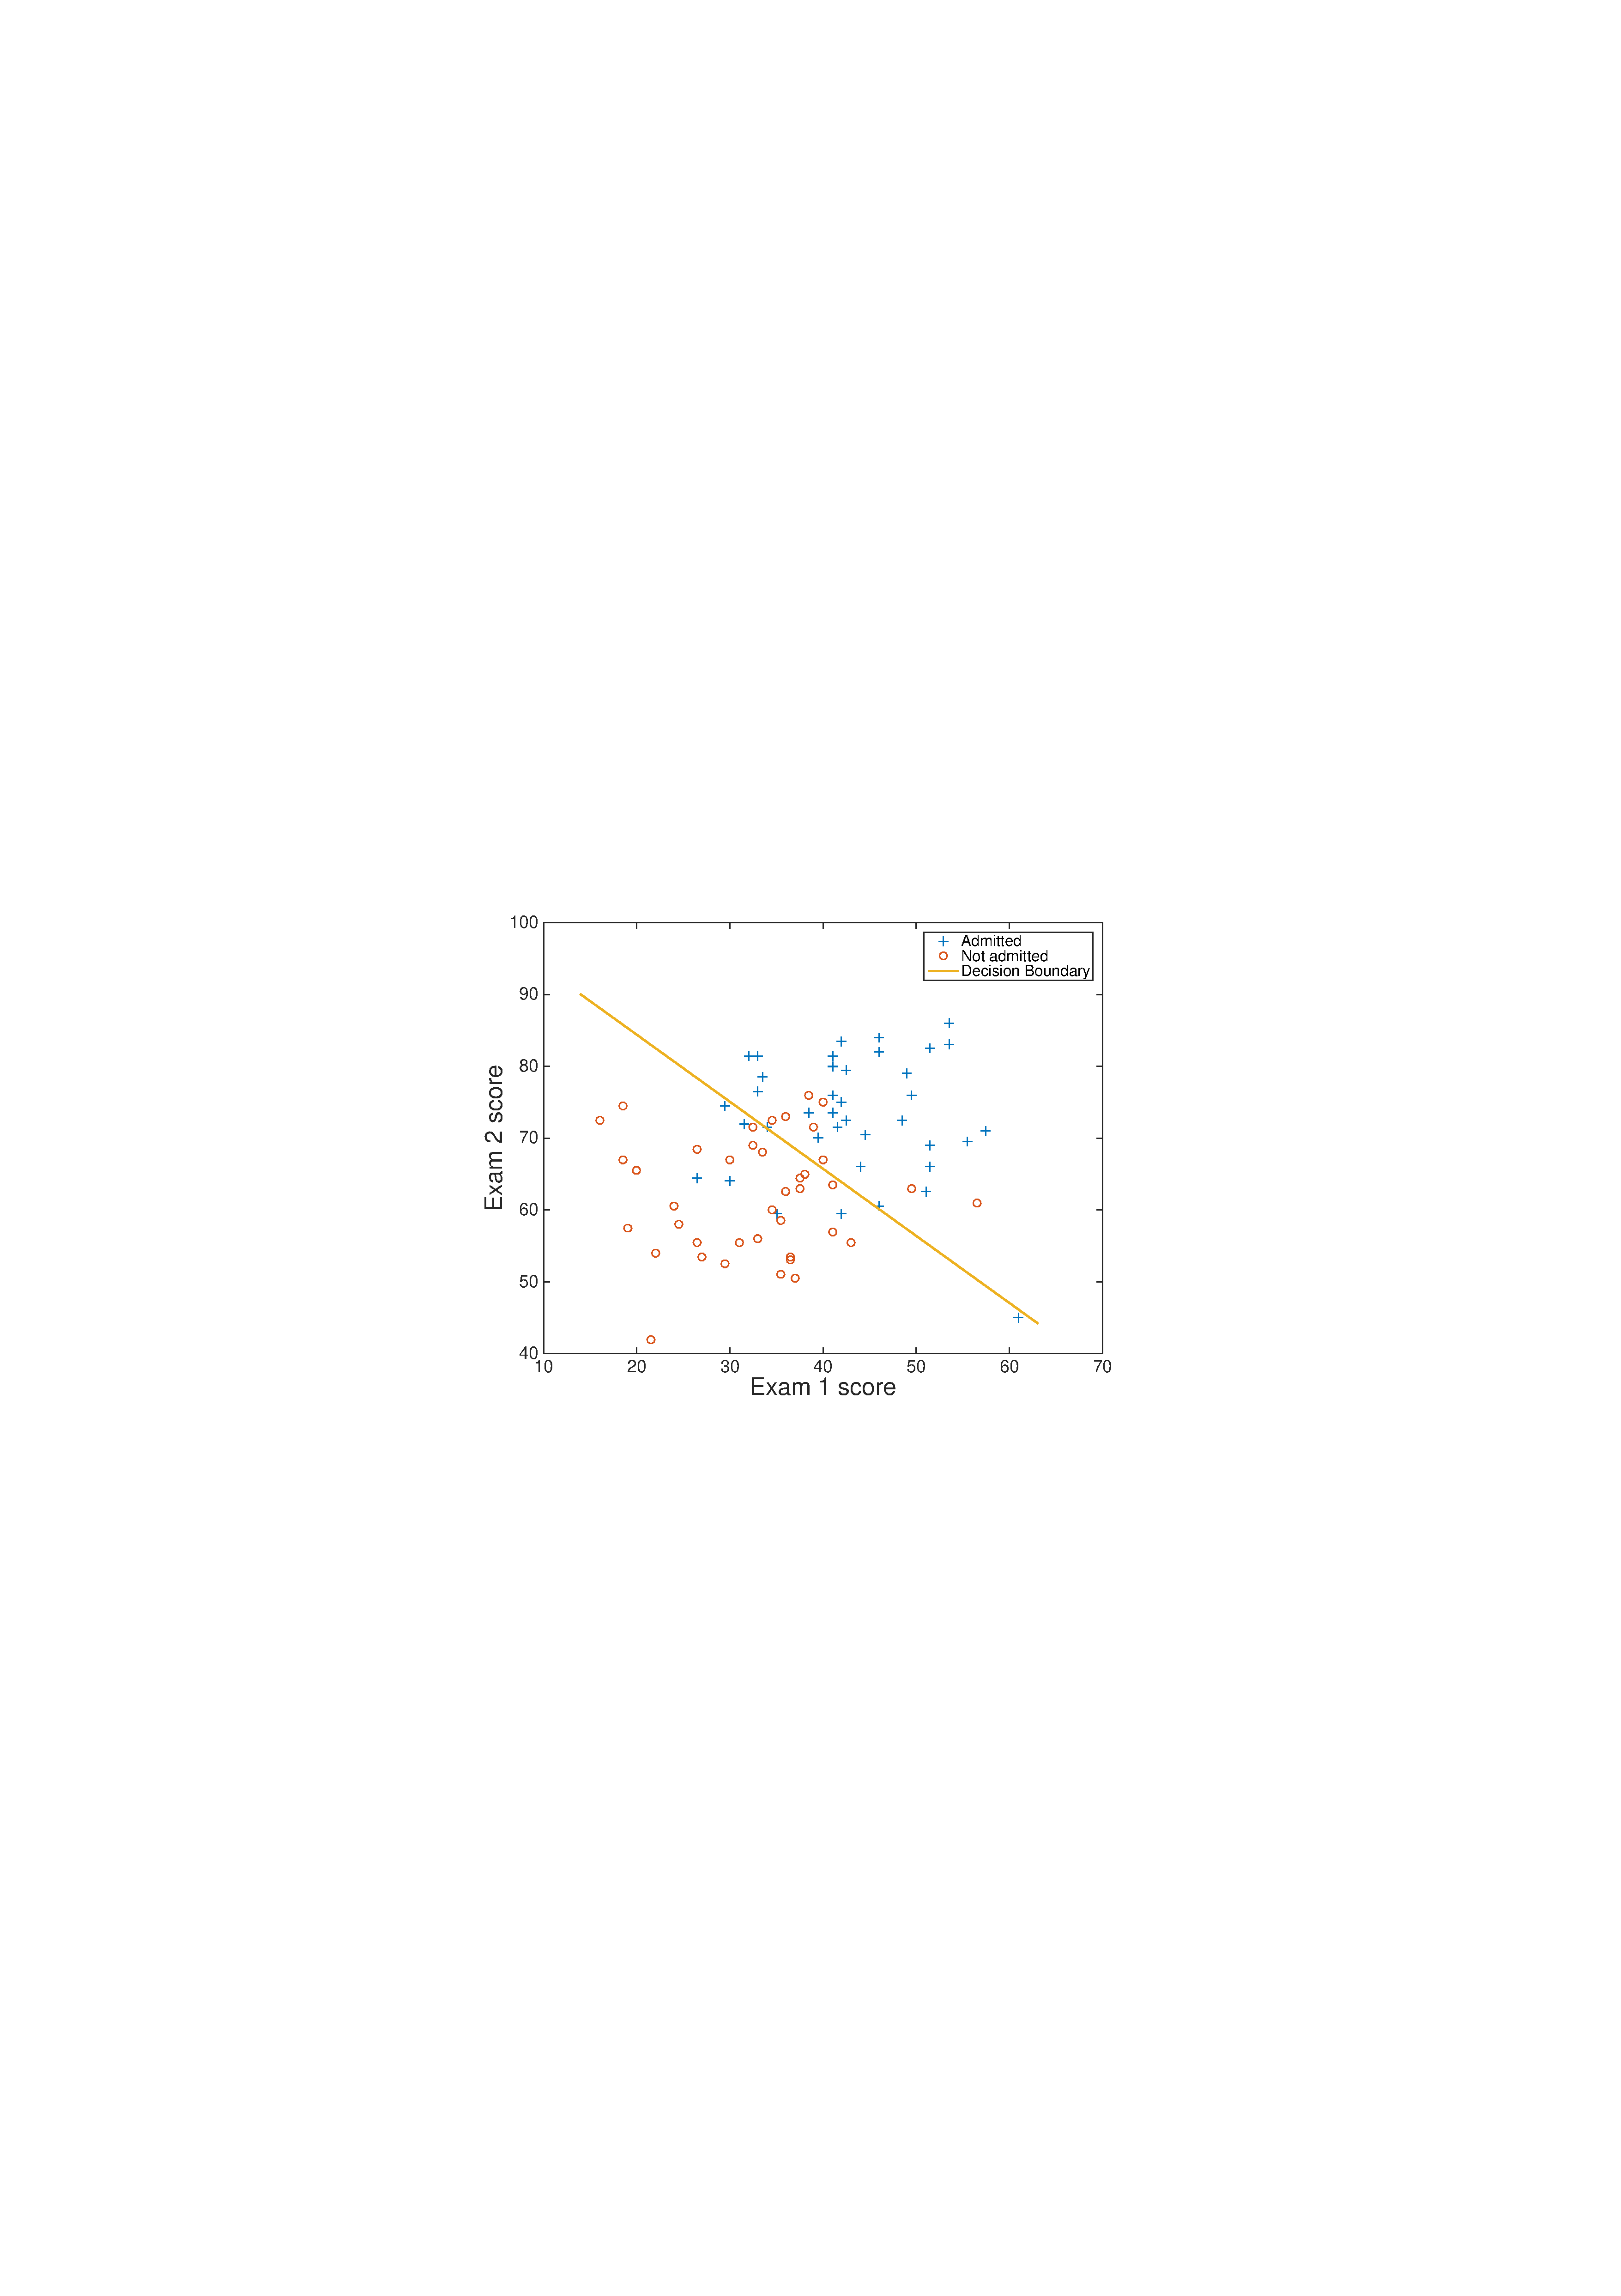
\includegraphics[width=.7\columnwidth]{data} \\ %\vspace{1ex}
  \caption{Data set and decision boundary.}
  \label{fig:data}
  \end{figure}


\section{Newton's Method}
%
  Through Newton's method, the final values of $\theta$ are $\theta_0 =  -16.3787$, $\theta_1=0.1483$, and $\theta_2=0.1589$. We show the convergence of the Newton's method in Fig.~\ref{fig:con}. It is demonstrated that, the Newton's method achieves convergence in only 5 iterations. Recall that, in our previous experiments, the gradient descent method took hundreds or even thousands of iterations to converge. The Newton's method is much faster.
  %
  \begin{figure}[htb!]
  \centering
    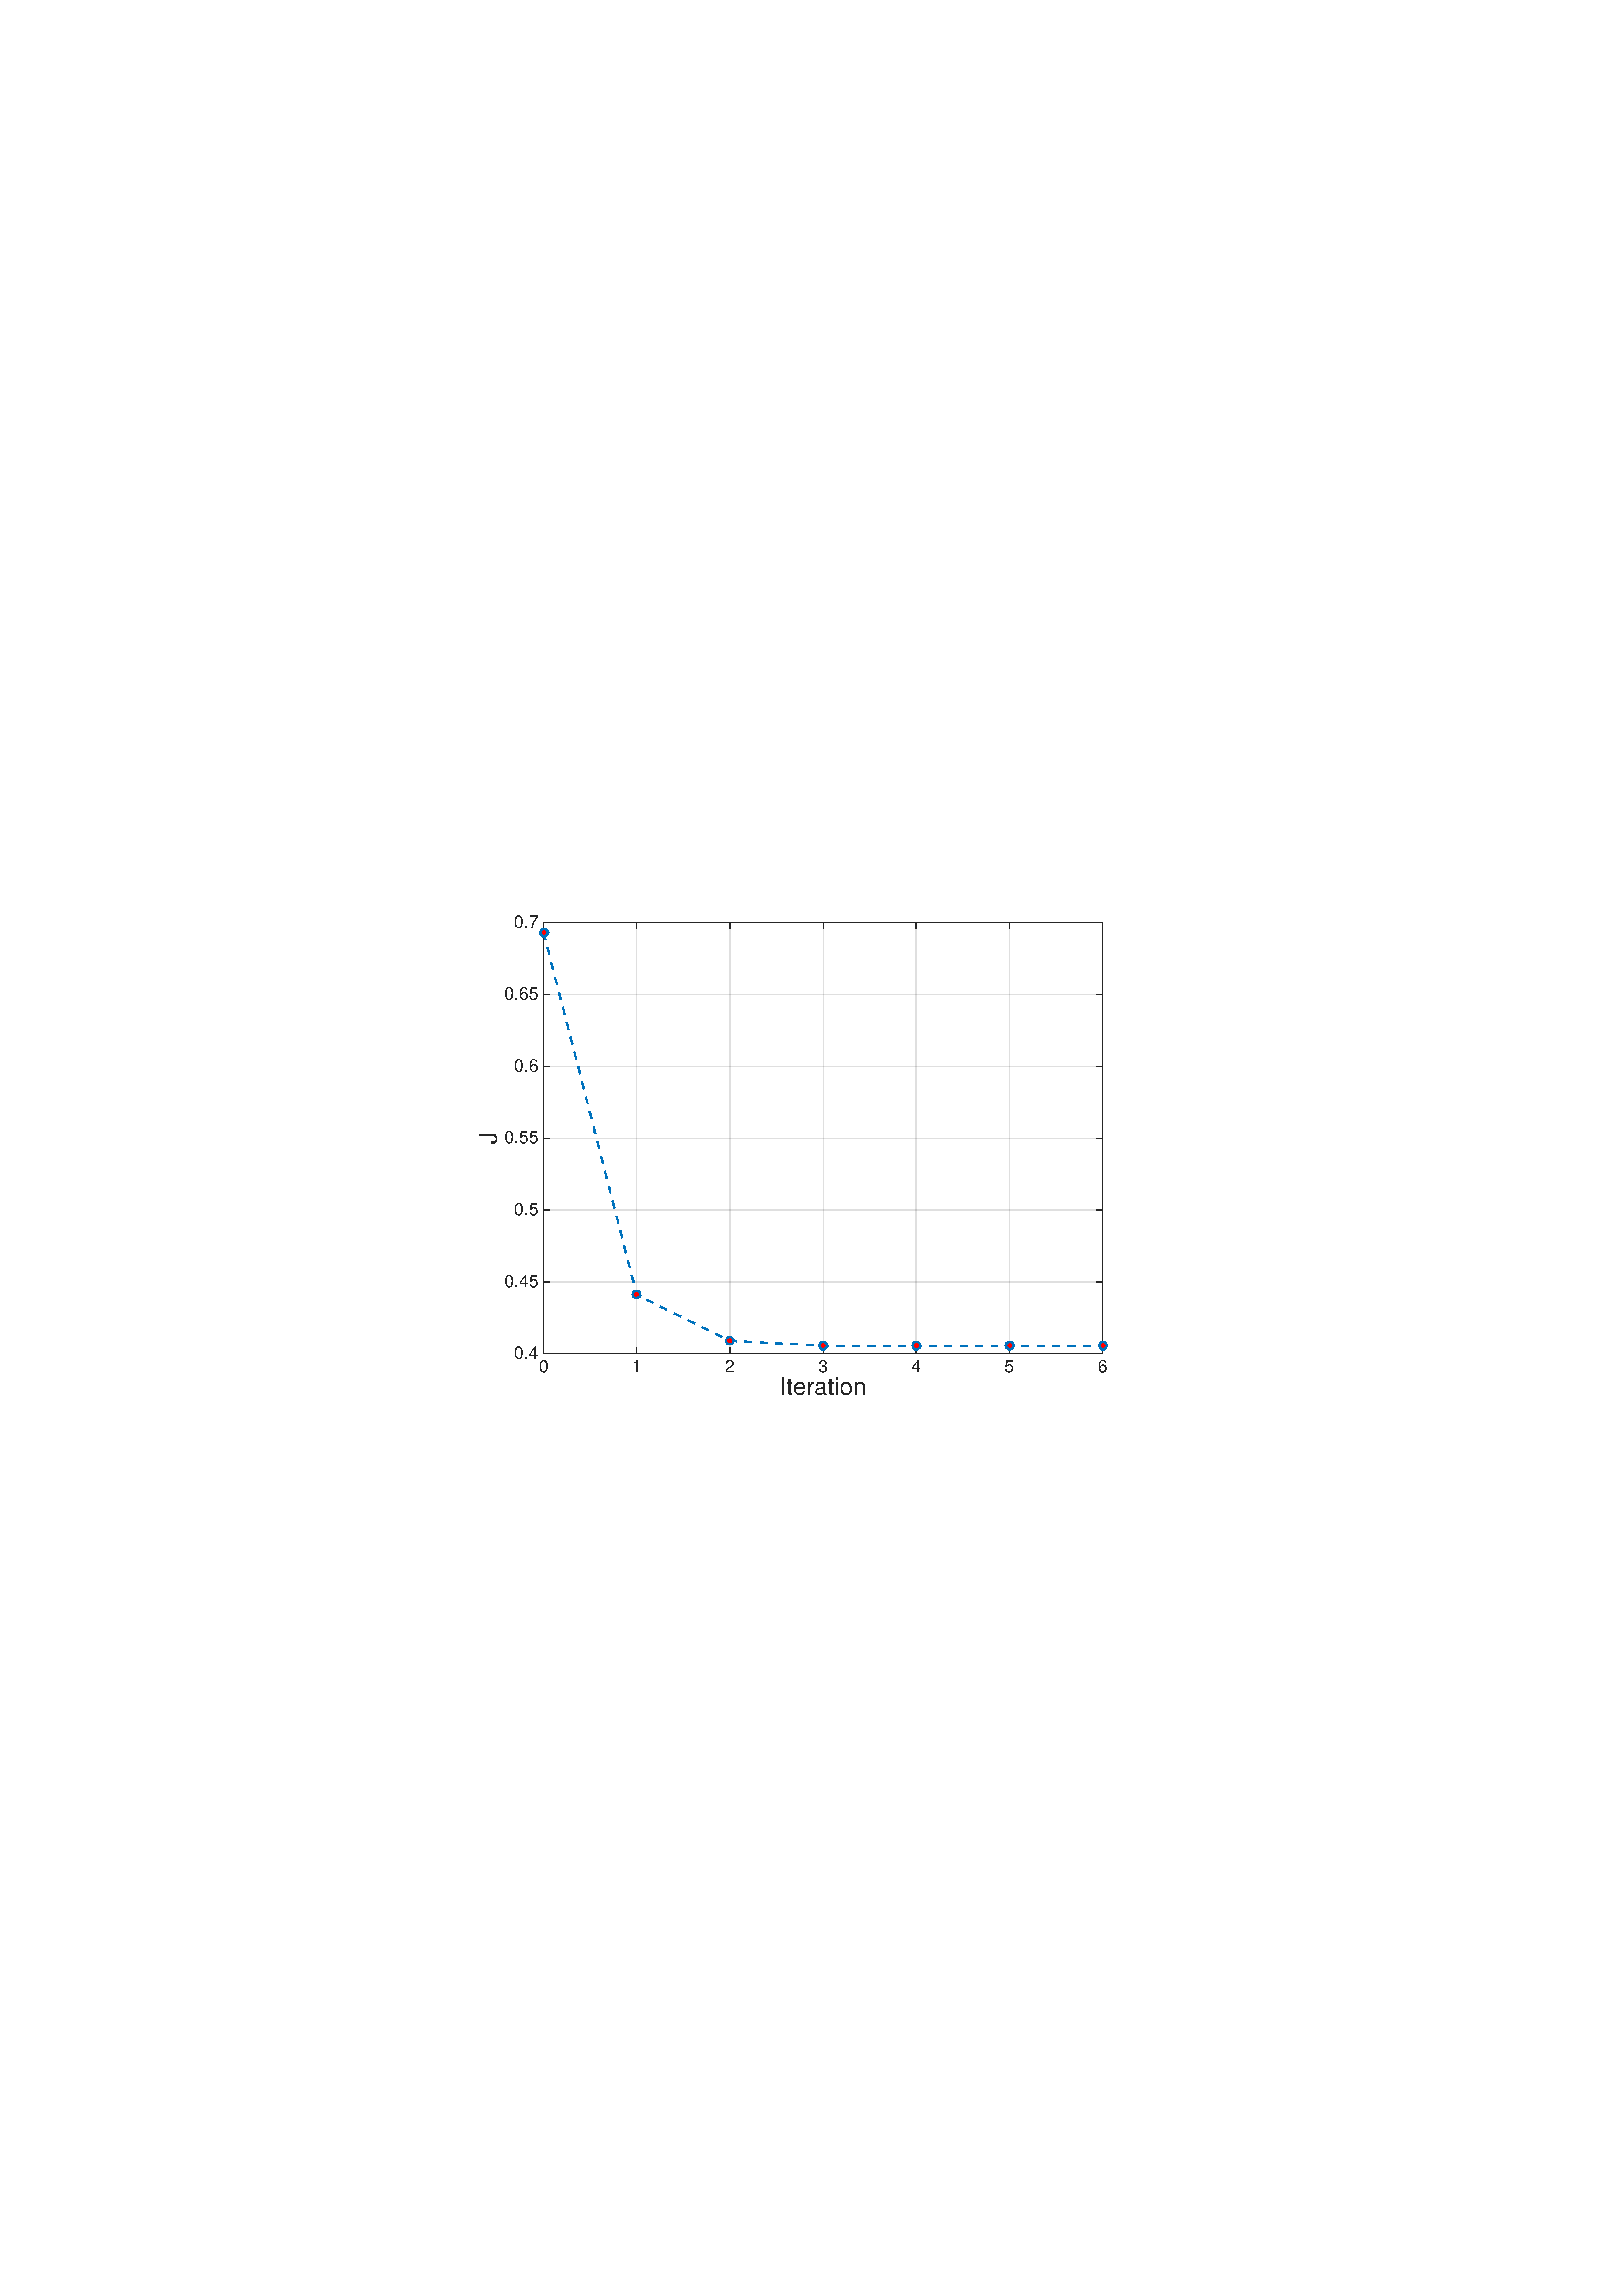
\includegraphics[width=.7\columnwidth]{convergence} \\ %\vspace{1ex}
  \caption{Convergence.}
  \label{fig:con}
  \end{figure}

\end{document}








  \end{lstlisting}
  %


